% make sure you have the VPN on, so that latex can load packages on the fly
% upload the project folder to overleaf

\documentclass[12pt,twoside]{scrreport}

\usepackage[a4paper,inner=1.5in,outer=1in,top=1in,bottom=1in]{geometry}

\usepackage{ipsum}

\usepackage{chngcntr} % Allows customization of counters
\counterwithout{figure}{chapter} % Make figure numbers independent of chapters
\counterwithout{table}{chapter}  % Make table numbers independent of chapters

\usepackage[printonlyused]{acronym}

% graphics package
\usepackage{graphicx} 

\usepackage[ngerman, english]{babel}

% enhanced citation package 
\usepackage{natbib}
\bibpunct{(}{)}{;}{a}{}{,}  % to adjust punctuation in references


% adjust caption properties
\usepackage{caption} 
\captionsetup[table]{position=top,justification=justified,singlelinecheck=false,format=plain}
\captionsetup[figure]{position=below,justification=justified,singlelinecheck=false,format=plain}

\captionsetup{
	labelfont=bf,         % Bold label (e.g., Table 2:)
	textfont=normalfont,  % Normal font for the text
	labelsep=colon,       % Colon after "Table X" or "Figure X"
	indention=0pt         % No indentation on the second and following lines
}



% hyperrefs on, with nicer colors
\usepackage{color}
\usepackage{xcolor}
\usepackage[]{hyperref}
\definecolor{darkblue}{rgb}{0,0,.5}
\hypersetup{colorlinks=true, breaklinks=true, linkcolor=darkblue, menucolor=darkblue, urlcolor=darkblue, citecolor=darkblue}

% enhanced tables
\usepackage{multicol}              
\usepackage{multirow}
\usepackage{booktabs} 

% For displaying code
\usepackage{listings}

\usepackage{tikz}

% Define custom settings for R code
%\lstset{
	%language=R,
	%basicstyle=\ttfamily\footnotesize,
	%showstringspaces=false,
	%breaklines=true,
	%frame=single,
	%numbers=left,
	%numberstyle=\tiny\color{gray},
	%captionpos=b
%}

% Commands for formatting R elements
\newcommand{\pkg}[1]{`#1'}
\newcommand{\fn}[2][]{\textit{#2(}#1\textit{)}}
\newcommand{\val}[1]{\texttt{#1}}


\usepackage{float}

%Tilde ~
\usepackage{textcomp}

%\setcounter{secnumdepth}{3}
%\setcounter{tocdepth}{4}
\begin{document}
\pagenumbering{gobble}
\begin{titlepage}
% Symmetrical margins for title page
\newgeometry{top=1in,bottom=1in,left=1in,right=1in} 
\selectlanguage{ngerman}
\begin{center}
% UR Logo
\begin{tikzpicture}[scale=0.5]
	\begin{pgfscope}
		\definecolor{eps2pgf_color}{RGB}{142,142,141}\pgfsetstrokecolor{eps2pgf_color}\pgfsetfillcolor{eps2pgf_color}
		\pgfpathmoveto{\pgfqpoint{2.5cm}{0cm}}
		\pgfpathcurveto{\pgfqpoint{3.881cm}{0cm}}{\pgfqpoint{5cm}{1.119cm}}{\pgfqpoint{5cm}{2.5cm}}
		\pgfpathcurveto{\pgfqpoint{5cm}{3.881cm}}{\pgfqpoint{3.881cm}{5cm}}{\pgfqpoint{2.5cm}{5cm}}
		\pgfpathcurveto{\pgfqpoint{1.119cm}{5cm}}{\pgfqpoint{0cm}{3.881cm}}{\pgfqpoint{0cm}{2.5cm}}
		\pgfpathcurveto{\pgfqpoint{0cm}{1.119cm}}{\pgfqpoint{1.119cm}{0cm}}{\pgfqpoint{2.5cm}{0cm}}
		\pgfusepath{fill}
		\definecolor{eps2pgf_color}{gray}{1}\pgfsetstrokecolor{eps2pgf_color}\pgfsetfillcolor{eps2pgf_color}
		\pgfpathmoveto{\pgfqpoint{3.023cm}{2.542cm}}
		\pgfpathlineto{\pgfqpoint{3.64cm}{2.542cm}}
		\pgfpathlineto{\pgfqpoint{3.64cm}{1.194cm}}
		\pgfpathcurveto{\pgfqpoint{3.64cm}{0.996cm}}{\pgfqpoint{3.67cm}{0.853cm}}{\pgfqpoint{3.728cm}{0.765cm}}
		\pgfpathcurveto{\pgfqpoint{3.787cm}{0.677cm}}{\pgfqpoint{3.881cm}{0.633cm}}{\pgfqpoint{4.01cm}{0.633cm}}
		\pgfpathcurveto{\pgfqpoint{4.143cm}{0.633cm}}{\pgfqpoint{4.243cm}{0.68cm}}{\pgfqpoint{4.31cm}{0.775cm}}
		\pgfpathcurveto{\pgfqpoint{4.377cm}{0.869cm}}{\pgfqpoint{4.411cm}{1.009cm}}{\pgfqpoint{4.411cm}{1.194cm}}
		\pgfpathlineto{\pgfqpoint{4.411cm}{2.542cm}}
		\pgfpathlineto{\pgfqpoint{5cm}{2.542cm}}
		\pgfpathlineto{\pgfqpoint{5cm}{1.194cm}}
		\pgfpathcurveto{\pgfqpoint{5cm}{0.853cm}}{\pgfqpoint{4.918cm}{0.597cm}}{\pgfqpoint{4.753cm}{0.426cm}}
		\pgfpathcurveto{\pgfqpoint{4.588cm}{0.257cm}}{\pgfqpoint{4.341cm}{0.172cm}}{\pgfqpoint{4.011cm}{0.172cm}}
		\pgfpathcurveto{\pgfqpoint{3.684cm}{0.172cm}}{\pgfqpoint{3.437cm}{0.257cm}}{\pgfqpoint{3.271cm}{0.428cm}}
		\pgfpathcurveto{\pgfqpoint{3.106cm}{0.6cm}}{\pgfqpoint{3.023cm}{0.855cm}}{\pgfqpoint{3.023cm}{1.194cm}}
		\pgfpathlineto{\pgfqpoint{3.023cm}{2.542cm}}
		\pgfusepath{fill}
		\definecolor{eps2pgf_color}{RGB}{142,142,141}\pgfsetstrokecolor{eps2pgf_color}\pgfsetfillcolor{eps2pgf_color}
		\pgfpathmoveto{\pgfqpoint{5cm}{2.544cm}}
		\pgfpathlineto{\pgfqpoint{5.921cm}{2.544cm}}
		\pgfpathcurveto{\pgfqpoint{6.228cm}{2.544cm}}{\pgfqpoint{6.455cm}{2.495cm}}{\pgfqpoint{6.603cm}{2.395cm}}
		\pgfpathcurveto{\pgfqpoint{6.752cm}{2.296cm}}{\pgfqpoint{6.826cm}{2.144cm}}{\pgfqpoint{6.826cm}{1.941cm}}
		\pgfpathcurveto{\pgfqpoint{6.826cm}{1.791cm}}{\pgfqpoint{6.787cm}{1.668cm}}{\pgfqpoint{6.708cm}{1.571cm}}
		\pgfpathcurveto{\pgfqpoint{6.63cm}{1.475cm}}{\pgfqpoint{6.517cm}{1.41cm}}{\pgfqpoint{6.37cm}{1.377cm}}
		\pgfpathcurveto{\pgfqpoint{6.491cm}{1.333cm}}{\pgfqpoint{6.589cm}{1.206cm}}{\pgfqpoint{6.663cm}{0.998cm}}
		\pgfpathlineto{\pgfqpoint{6.663cm}{0.996cm}}
		\pgfpathlineto{\pgfqpoint{6.94cm}{0.228cm}}
		\pgfpathlineto{\pgfqpoint{6.296cm}{0.228cm}}
		\pgfpathlineto{\pgfqpoint{6.093cm}{0.863cm}}
		\pgfpathcurveto{\pgfqpoint{6.06cm}{0.964cm}}{\pgfqpoint{6.015cm}{1.035cm}}{\pgfqpoint{5.959cm}{1.075cm}}
		\pgfpathcurveto{\pgfqpoint{5.902cm}{1.113cm}}{\pgfqpoint{5.814cm}{1.133cm}}{\pgfqpoint{5.695cm}{1.133cm}}
		\pgfpathlineto{\pgfqpoint{5.605cm}{1.133cm}}
		\pgfpathlineto{\pgfqpoint{5.605cm}{0.228cm}}
		\pgfpathlineto{\pgfqpoint{5cm}{0.228cm}}
		\pgfpathclose
		\pgfpathmoveto{\pgfqpoint{5.605cm}{2.137cm}}
		\pgfpathlineto{\pgfqpoint{5.605cm}{1.543cm}}
		\pgfpathlineto{\pgfqpoint{5.822cm}{1.543cm}}
		\pgfpathcurveto{\pgfqpoint{5.956cm}{1.543cm}}{\pgfqpoint{6.056cm}{1.567cm}}{\pgfqpoint{6.123cm}{1.616cm}}
		\pgfpathcurveto{\pgfqpoint{6.189cm}{1.664cm}}{\pgfqpoint{6.223cm}{1.737cm}}{\pgfqpoint{6.223cm}{1.834cm}}
		\pgfpathcurveto{\pgfqpoint{6.223cm}{1.938cm}}{\pgfqpoint{6.185cm}{2.015cm}}{\pgfqpoint{6.111cm}{2.064cm}}
		\pgfpathcurveto{\pgfqpoint{6.037cm}{2.113cm}}{\pgfqpoint{5.919cm}{2.137cm}}{\pgfqpoint{5.758cm}{2.137cm}}
		\pgfpathlineto{\pgfqpoint{5.605cm}{2.137cm}}
		\pgfusepath{fill}
	\end{pgfscope}
\end{tikzpicture}

\vfill

{\LARGE \textbf{Extending the \pkg{cito} package: deep convolutional neural networks in ecology}}

\vfill

{\LARGE \textbf{Masterarbeit}}

\vspace{0.5cm}
\large
zur Erlangung des akademischen Grades\\
Master of Science\\
in Computational Science\\
an der Fakultät für Physik\\
der Universität Regensburg
\vfill

\end{center}

\begin{tabular}{ll}
%Eingereicht bei: & Prof.\ Dr.\ Florian Hartig \\
%& Lehrstuhl für Theoretische Ökologie \vspace{5mm}\\

Vorgelegt von: & Armin Schenk \\
& Matrikelnummer: 2037367 \\
& E-Mail: \url{armin.schenk@stud.uni-regensburg.de} \vspace{5mm}\\

Erstgutachter: & Prof. Dr. Florian Hartig\\
Zweitgutachter: & Prof. Dr. Rainer Spang \vspace{5mm}\\

Eingereicht am: & \today\\
\end{tabular}
% Restore original margins
\restoregeometry 
\end{titlepage}

\thispagestyle{empty}
\vspace*{\fill} % Push content to the bottom of the page
\mbox{} % Add an invisible box (to ensure the page is recognized as non-empty)
\selectlanguage{english}

\chapter*{Abstract}
\noindent In recent years, there has been a growing interest in convolutional neural networks (CNNs) in the field of ecology. Typically, extensive deep learning frameworks, such as PyTorch or Tensorflow, are used to build and train these models. However, using these frameworks requires considerable expertise and time. Here, I present an extension to the R package \pkg{cito} that allows novice users to build and train CNNs with minimal code. The \pkg{cito} package is based on the numerically optimized \pkg{torch} backend, which allows efficient training of CNNs on graphics processing units (GPUs). In addition, several CNNs pre-trained on the large ImageNet dataset are available in \pkg{cito} for transfer learning. Moreover, I implemented a function that combines fully-connected neural networks and CNNs into a multimodal neural network (MMN). This allows a single network to be trained on and process several different types of data. I demonstrate the new features of \pkg{cito} with the example of bird species classification based on bird calls. My hope is that by providing a user-friendly pipeline for building and training CNNs and MMNs, these complex model architectures will become more accessible to researchers in the field of ecology.
\newline\newline
Keywords: convolutional neural network, multimodal neural network, machine learning, deep learning, transfer learning, R language, classification, regression
\vspace{3cm}
\section*{Acknowledgments}
I would like to thank Prof. Dr. Florian Hartig for supervising my thesis and always taking the time to discuss my work and provide feedback. Special thanks also to Dr. Maximilian Pichler for all his help and feedback, especially regarding the design choices of \pkg{cito}. I would also like to thank my friend Christian for all his encouragement throughout my studies.

\newpage
\thispagestyle{empty}
\vspace*{\fill} % Push content to the bottom of the page
\mbox{} % Add an invisible box (to ensure the page is recognized as non-empty)

\tableofcontents

\newpage
\thispagestyle{empty}
\vspace*{\fill} % Push content to the bottom of the page
\mbox{} % Add an invisible box (to ensure the page is recognized as non-empty)

\chapter*{Introduction}
\addcontentsline{toc}{chapter}{Introduction}
\pagenumbering{arabic}
\setcounter{page}{1}
In recent years, deep neural networks have made remarkable breakthroughs across diverse scientific fields \citep{jordanMachineLearningTrends2015}. In computer vision, models like Mask R-CNN \citep{heMaskRCNN2017} have revolutionized object detection in images. In autonomous driving, deep learning has become essential for navigation and decision-making \citep{bojarskiEndEndLearning2016}. AlphaZero \citep{silverMasteringChessShogi2017} demonstrated superhuman levels of play in strategic games such as chess, shogi and go, while AlphaFold \citep{jumperHighlyAccurateProtein2021} solved the long-standing challenge of predicting the 3D structure of proteins from their amino acid sequence. In natural language processing, large language models \citep[e.g., GPT-3,][]{brownLanguageModelsAre2020} enabled applications like sentiment analysis, text summarization and conversational AI such as ChatGPT (\url{https://chat.openai.com}). This progress in deep learning has been driven by the ever-increasing availability of data and computing resources, as well as advances in learning algorithms and network architectures, such as transformers \citep{vaswaniAttentionAllYou2017}.

Deep learning has also found widespread applications in ecology, advancing tasks such as species distribution modeling, prediction of species interactions, and ecosystem monitoring \citep{chenEndEndLearningDeep2018, wilkinsonComparisonJointSpecies2019, pichlerMachineLearningAlgorithms2020, pichlerMachineLearningDeep2023, borowiecDeepLearningTool2022, tuiaPerspectivesMachineLearning2022, christinApplicationsDeepLearning2019}. While traditionally scalar data such as climate variables, soil properties or species traits have been used to address ecological questions, the growing availability of structured data is transforming the field. Modern monitoring technologies, including camera traps, aerial drones, satellites, and acoustic sensors, generate large datasets in the form of images, videos, and audio recordings. Most of the information in these datasets lies in their spatial or temporal structure, making it crucial to use specialized architectures that can capture these patterns effectively. Convolutional neural networks \citep[CNNs,]{lecunBackpropagationAppliedHandwritten1989a}, designed to detect and hierarchically combine spatial features, have thus become the most widely used network architecture in ecological applications. They have been applied to tasks such as automatic species recognition, biodiversity monitoring, habitat mapping, land cover classification, and the detection of invasive species (\citep{gomezvillaAutomaticWildAnimal2017, norouzzadehAutomaticallyIdentifyingCounting2018, tabakMachineLearningClassify2019, salamonFusingShallowDeep2017, liDeepLearningRemote2018, kattenbornConvolutionalNeuralNetworks2019, qianUAVDeepConvolutional2020}.

At the core of CNNs are convolutional layers that apply small, localized filters (also called kernels) that scan across the input to capture patterns such as edges, textures, and shapes. Subsequent convolutional layers then combine these patterns hierarchically, allowing the CNN to capture increasingly complex patterns such as objects and people. CNNs also often use pooling layers (e.g. max-pooling) to downsample the resulting feature maps by combining values in local regions while retaining significant information. This not only makes the network more computationally efficient, but also helps to avoid overfitting problems \citep{liSurveyConvolutionalNeural2022}.

More recently, even multimodal neural networks (MMNs) have been used in ecology. MMNs combine different neural network architectures to extract and combine features from different data types. For example, an MMN consisting of a dense neural network (DNN) and a CNN can be used to process tabular data (e.g. environmental variables) and image data (e.g. satellite images) at the same time \citep{zhangNovelMultimodalSpecies2022, hu2024introduction}.

CNNs and MMNs, like most state-of-the-art networks, are typically built using extensive deep learning frameworks such as \pkg{TensorFlow} \citep{abadiTensorFlowSystemLargeScale2016} and \pkg{PyTorch} \citep{paszkePyTorchImperativeStyle2019}, which offer powerful tools for building and training sophisticated models. However, these frameworks, while highly flexible and efficient, are notoriously difficult to use due to their complexity and steep learning curve. To address this problem, several frontends have been developed with the aim to simplify their usage, including the popular R (\url{www.r-project.org}) frontends \pkg{keras} \citep{chollet2015keras} for TensorFlow and \pkg{luz} \citep{falbelLuzHigherLevel2024} for PyTorch. Despite these efforts, these frontends remain challenging to use, especially for ecologists that are accustomed to the intuitive and user-friendly design of other R packages used for statistical analysis. For instance, packages such as \pkg{ranger} and \pkg{lme4} allow traditional machine learning models like random forest and statistical models like mixed-effect models to be fitted in a single line of code.

Several R packages have been developed with the goal to imitate this user-friendly design for deep learning. Of these packages, \pkg{cito} \citep{amesoderCitoPackageTraining2024} stands out in particular. Not only does it provide a user-friendly interface to build and train deep neural networks in a single line of code, it also provides many important functionalities ranging from regularization techniques that control the bias-variance trade-off (e.g., elastic net regularization, dropout) to modern training techniques that help with convergence (e.g., early stopping, learning rate scheduler). \pkg{cito} uses \pkg{torch} \citep{falbelTorchTensorsNeural2024}, a native implementation of the PyTorch framework in R, as backend, taking full advantage of its numerically optimized functions and the integrated support of graphic processing units (GPUs), which is crucial for the efficient training of large neural networks.

However, the current version of \pkg{cito} only supports dense neural networks (DNNs), an architecture in which every input neuron is connected to every neuron in subsequent layers. By design, DNNs are invariant to the positional arrangement of input features, which makes them work best on unstructured, tabular data, but also unsuitable for spatially structured data, such as images, where the relationships between neighboring pixels contain crucial information. As a result, \pkg{cito} is unable to address the ecological tasks that arose with the trend of spatially structured data.

Here, I present the new implementations of CNNs and MMNs in the \pkg{cito} package. In line with the design philosophy of \pkg{cito}, I provide user-friendly functions that allow building and training CNNs and MMNs with minimal code, while also offering a high degree of customization. In addition to the functionalities known from the DNN implementation of \pkg{cito}, such as GPU support, deep learning techniques (e.g., regularization, learning rate scheduler) and downstream functionalities (e.g. continuing training, architecture visualization), I also implemented the option to use pre-trained models for transfer learning. This makes \pkg{cito} the first R package, that allows building and training CNNs and MMNs as intuitively as other R packages do for traditional methods like random forest.

In the remainder of this work, I introduce the new functions, discuss design choices and validation, and demonstrate the new possible applications of \pkg{cito} using the example of bird species classification based on audio data.

\chapter*{Introducing the \pkg{cito} \fn{cnn} function}
\addcontentsline{toc}{chapter}{Introducing the \pkg{cito} \fn{cnn} function}
Overview

\section*{Specifying CNN architectures}
\addcontentsline{toc}{section}{Specifying CNN architectures}

The first step in building any neural network is to specify its architecture. For DNNs, this is done within \pkg{cito}s \fn{dnn} function, by providing three vectors (\val{hidden}, \val{activation} and \val{bias}). Since the architecture of CNNs is much more complex, the specification of the desired architecture is done in a separate function called \fn{create\_architecture}, which returns an object describing the architecture, which can then be passed to the new \fn{cnn} function, which we will discuss later. This is done to make the use of CNNs as user-friendly as possible, by not overloading a single function call with too many arguments and instead clearly separating them into arguments related to architecture and training, respectively. The function call of the \fn{create\_architecture} function looks like this:

\begin{figure}[h]
	\centering
	\newsavebox{\lstbox} % Create a savebox to store the listing
	\begin{lrbox}{\lstbox}
		\begin{lstlisting}
create_architecture <- function(...,
  default_n_neurons = 10,
  default_n_kernels = 10,
  default_kernel_size = list(conv = 3, maxPool = 2, avgPool = 2),
  default_stride = list(conv = 1, maxPool = NULL, avgPool = NULL),
  default_padding = list(conv = 0, maxPool = 0, avgPool = 0),
  default_dilation = list(conv = 1, maxPool = 1),
  default_bias = list(conv = TRUE, linear = TRUE),
  default_activation = list(conv = "relu", linear = "relu"),
  default_normalization = list(conv = FALSE, linear = FALSE),
  default_dropout = list(conv = 0.0, linear = 0.0))
		\end{lstlisting}
	\end{lrbox}
	\resizebox{\textwidth}{!}{\usebox{\lstbox}}
\end{figure}

The core structure of a CNN consists of a combination of convolutional and pooling layers, followed by one or more linear layers. These layers can be specified using the provided layer functions \fn{conv}, \fn{avgPool}, \fn{maxPool} and \fn{linear}, and then passed to the \fn{create\_architecture} function, which combines them into a complete architecture. Each of these functions has several arguments (see Table \ref{layers}) that affect the corresponding layer, but can also be used without specifying any of them. In this case, the unspecified arguments are filled with the default values set within the \fn{create\_architecture} function. For example, a linear layer created with \fn[\val{n\_neurons=128}]{linear} will have its unspecified arguments \val{bias}, \val{activation}, \val{normalization} and \val{dropout} set to \val{TRUE}, \val{"relu"}, \val{FALSE} and \val{0.0} respectively. These defaults can be overridden in the \fn{create\_architecture} function. For example, if you want to introduce a dropout rate of \val{0.5} for all linear layers that don't specify the dropout rate themselves, you can set \val{default\_dropout = }\fn[\val{linear=0.5}]{list}. Note that this only changes the default value for linear layers, leaving the default dropout rate for convolutional layers at \val{0.0}. If you don't want this, you can either also set a different default for convolutional layers (e.g. \val{default\_dropout = }\fn[\val{linear=0.5, conv=0.3}]{list}) or set the default dropout rate for both linear and convolutional layers to the same value with \val{default\_dropout = 0.5}. This implementation of the \fn{create\_architecture} function allows a high degree of flexibility and customization, while still allowing users who don't need it to specify CNN architectures in a single line of code (see section \pkg{Case study}).

\begin{table}[t]
	\caption{Functions that specify the layers for the \fn{create\_architecture} function. The arguments configure the architecture of the corresponding layer and the defaults are set to commonly used values. However, the architecture of the network and each layer is usually tuned for better performance. In particular, the n\_kernels argument shouldn't be the same for all convolutional layers of the network. It's common practice to increase n\_kernels the deeper the convolutional layer is in the network. Additionally, the linear and convolutional layers include the normalization and dropout parameters, which are used to add batch normalization and dropout regularization to the corresponding layer.}
	\centering
	%\renewcommand{\arraystretch}{1.3}
	\resizebox{\textwidth}{!}{
		\begin{tabular}{|llll|}
			\hline
			\textbf{Function}                                & \textbf{Arguments}     & \textbf{Explanation}                                                                                                                       & \textbf{Default}   \\ \hline
			
			\multirow{9}{*}{\textbf{conv()}}     & n\_kernels    & Number of kernels                                                                                                  & 10        \\
			& kernel\_size  & Size of kernels                                                                           & 3         \\
			& stride        & Stride of kernels                                                                     & 1         \\
			& dilation      & Dilation of kernels                                                                 & 1         \\
			& padding       & Zero-padding applied to input                                        & 0         \\
			& bias          & Add bias to kernels                                                              & TRUE      \\
			& activation    & Activation function                                         & 'relu'    \\
			& normalization & Add batch normalization to output                                                      & FALSE     \\
			& dropout       & Dropout probability of output channels                          & 0         \\ \hline
			\multirow{3}{*}{\textbf{avgPool()}}  & kernel\_size  & Size of average-pooling window                                                                                                    & 2         \\
			& stride        & Stride of average-pooling window                                                                                                  & 2         \\
			& padding       & Zero-padding applied to input                                     & 0         \\ \hline
			\multirow{4}{*}{\textbf{maxPool()}}  & kernel\_size  & Size of maximum-pooling window                                                                                                    & 2         \\
			& stride        & Stride of maximum-pooling window                                                                                                  & 2         \\
			& dilation      & Dilation of maximum-pooling window                                                                                                & 1         \\
			& padding       & Zero-padding applied to input                                     & 0         \\
			\hline
			\multirow{5}{*}{\textbf{linear()}}   & n\_neurons    & Number of neurons                                                                                              & 10        \\
			& bias          & Add bias to neurons                                                              & TRUE      \\
			& activation    & Activation function                                                      & 'relu'    \\
			& normalization & Add batch normalization to output                                                      & FALSE     \\
			& dropout       & Dropout probability of neurons                                          & 0         \\ \hline
		\end{tabular}
	}

	\label{layers}
\end{table}

For the defaults, I have chosen values that are commonly used and make sense as defaults. For example, there are several things to consider when choosing the default kernel size: First, the kernel size should be greater than 1 so that the layer increases the receptive field of the CNN. This makes sense for a default value, but doesn't mean that a kernel size of 1 should never be used. For example, many popular architectures use kernels of size 1 for dimension reduction. The default kernel size should also be odd, so that it is possible to add symmetrical padding to make the output feature maps have the same size as the input feature maps. This is important for tasks that require precise spatial alignment, such as segmentation or detection [Zitat]. Finally, it has been shown that stacking multiple smaller convolutions achieves the same receptive field as a larger convolution, while being computationally cheaper (especially for 2D and 3D convolutions) and introducing more non-linearities [Zitat]. For example, two 3x3 convolutions achieve the same receptive field as a 5x5 convolution, but need only 18 parameters instead of 25. Therefore, 3 - as the smallest, odd number greater than 1 - is a suitable default value. This can also be seen in architectures such as VGGNet [Zitat] and ResNet [Zitat], which consist almost entirely of 3x3 convolutions.

To help the user understand the architecture created by the \fn{create\_architecture} function, I implemented \fn{print} and \fn{plot} functions for the resulting R object. These visualize the configuration of each layer in detail, including how the size of the input changes after each layer (Figure \ref{plot}).

\begin{table}[t]
	\caption{Arguments of the \fn{cnn} function that control the learning process of the network. The defaults are set to reasonable values, but hyperparameters (e.g. learning rate, batchsize, lambda and alpha) usually need to be tuned to avoid convergence problems and improve performance. Detailed guidance on this can be found in the \pkg{cito} R package \fn["Training neural networks"]{vignette}.}
	\centering
	%\renewcommand{\arraystretch}{1.1}
	\resizebox{\textwidth}{!}{
		\begin{tabular}{|lll|}
			\hline
			\textbf{Argument} & \textbf{Explanation}                                                                               & \textbf{Default} \\
			\hline
			%			loss               & Loss function                                                                             & 'mse'   \\
			optimizer          & Optimizer                                                                                 & 'sgd'   \\
			lr                 & Learning rate                                                                             & 0.01    \\
			lr\_scheduler      & Learning rate scheduler                                                                   & NULL    \\
			epochs             & Number of training epochs                                                                 & 100     \\
			early\_stopping    & Stop training early, if loss doesn't improve over specified number of epochs & Inf    \\
			burnin             & Stop training early, if loss isn't below base-loss after specified number of epochs    & Inf     \\
			validation         & Split data into training and validation set to monitor training                           & 0.0     \\
			batchsize          & Number of samples used in each training step                                              & 32      \\
			shuffle            & Shuffle training batches in between epochs                                                & TRUE    \\
			lambda             & Strength of elastic net regularization                                                    & 0       \\
			alpha              & Split of L1 and L2 regularization                                                         & 0.5     \\
			\hline
		\end{tabular}
	}
	
	\label{parameters}
\end{table}

\section*{Training CNNs and transfer learning}
\addcontentsline{toc}{section}{Training CNNs and transfer learning}
Once the architecture is specified, the network can be constructed and trained using the \fn{cnn} function. This function returns the trained network as an S3 object which contains not only the trained model itself, but also metadata about the architecture and training process. The S3 object can then be used to generate predictions on new data sets using the \fn{predict} function, or to continue training for additional epochs using the \fn{continue\_training} function. The latter also allows the training data and hyperparameters to be changed for further optimization. Additionally, the \fn{print} and \fn{plot} functions mentioned above are compatible with this object.

The arguments of the \fn{cnn} function include several hyperparameters (Table \ref{parameters}) that influence the training process and the performance of the network. These hyperparameters can be crucial to avoid common problems such as overfitting. For example, early stopping can be used to stop the training process early if the validation loss does not improve over a specified number of epochs, thus saving the network from unnecessary overtraining. Similarly, elastic net regularization, controlled by the lambda and alpha parameters, can help avoid overfitting by reducing the functional complexity of the network. However, improper configuration of the hyperparameters can also lead to reduced model performance and slow or even prevent convergence during training. While the defaults are set to values that should work for many applications, optimal performance typically requires tuning both the CNN architecture and the training hyperparameters, ideally under cross-validation. During training, \pkg{cito} visualizes both training and validation loss, allowing users to monitor the training process in real time. As an additional reference for comparison, the loss of an intercept-only model is depicted as a baseline. This visualization helps the user to identify potential problems such as lack of convergence or overfitting.

Training deep neural networks from scratch often requires large amounts of data, computational resources and time. In many applications, it can be useful to use a model that has already  been pre-trained on a large dataset from another task instead. The learned features of this network act as a good starting point and are fine-tuned during the training on the new dataset, to adapt the model to the task at hand. This not only minimizes the need for large datasets but also reduces the time required to train a network.

The R package \pkg{torchvision} provides several models pre-trained on the ImageNet dataset [Zitat], such as ResNet [Zitat] and MobileNet [Zitat]. To use the architectures of these models in \pkg{cito}, the user can use the \fn{transfer} function within the \fn{create\_architecture} function. In the \fn{transfer} function, the user specifies the name of the architecture to be used and whether the pre-trained parameters should be frozen, in which case only the parameters of the linear layers at the end of the network are adjusted during training. It is also possible to initialize these architectures with random parameters instead.

\section*{Multimodal neural networks}
\addcontentsline{toc}{section}{Multimodal neural networks}

\begin{figure}
	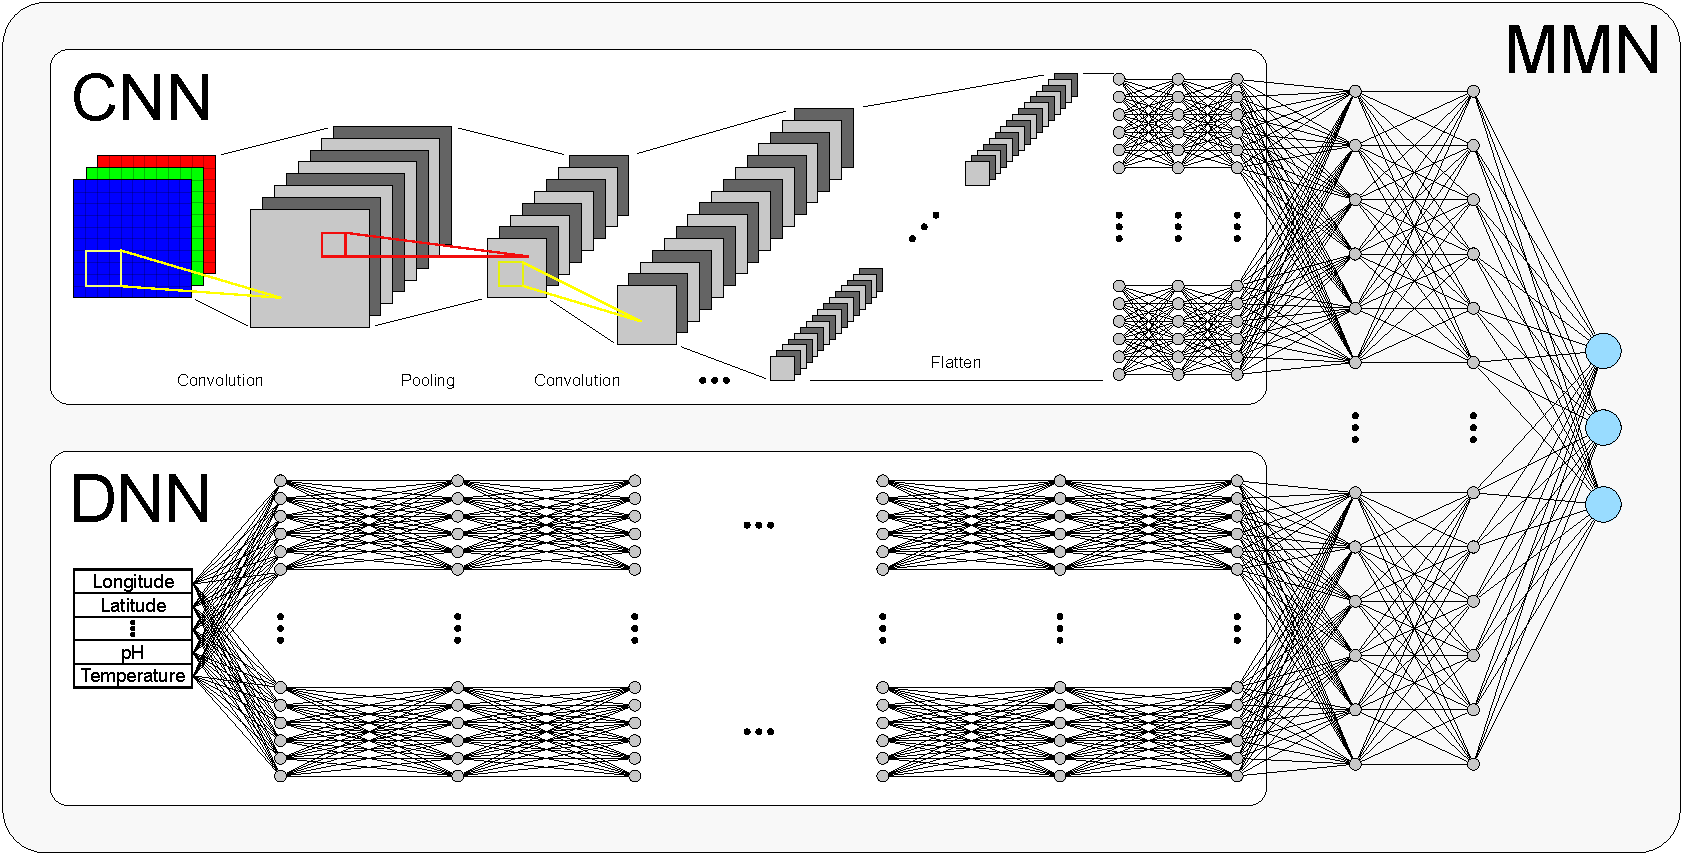
\includegraphics[width=\textwidth]{MMN.pdf}
	\label{MMN}
	\caption{Example of a multimodal neural network that combines a CNN and a DNN to process RGB images and tabular data in the same network. A network like this can be created by $mmn(Y \sim cnn(...) + dnn(...), ...)$. The \fn{mmn} function can combine any number of CNNs and DNNs.}
\end{figure}

Multimodal neural networks are designed to process data in different formats (e.g. image, tabular, sound) simultaneously. To do this, an appropriate architecture is built for each input format (e.g. CNN for image data, DNN for tabular data). The concatenated output embeddings of each of these architectures serve as input to a linear classifier that combines the different architectures. This allows the network to be trained on all data simultaneously, and to learn interactions between different data types.

MMNs are implemented in \pkg{cito} with the \fn{mmn} function, which allows the creation of MMNs combining any number of CNNs and DNNs. This can be specified by the user with a formula. For example, to create an MMN that consists of one CNN and one DNN:

\begin{lstlisting}[literate={~}{{$\sim$}}1]
	mmn(Y ~ cnn(...) + dnn(...), ...)
\end{lstlisting}

where Y is the response data. Within the \fn{cnn} and \fn{dnn} functions, the input data and the architecture of the corresponding subnetwork can be specified. The architecture of the linear classifier and the training hyperparameters (Table \ref{parameters}) can be specified in the \fn{mmn} function in the same way as in the \fn{dnn} function.

In the future, more neural network architectures (e.g. recurrent neural networks) are planned to be implemented in \pkg{cito}, which will allow the \fn{mmn} function to combine even more types of data. 

\section*{Package validation}
\addcontentsline{toc}{section}{Package validation}
To test the implementation of CNNs and MMNs, I designed unit tests using the R package \pkg{testthat} [Zitat]. The first tests check whether the architectures work for all possible combinations of input data, loss function and training device. To do this, I generate six randomly distributed input data sets to simulate the cases of 1D (e.g. spectrograms), 2D (e.g. images) and 3D (e.g. time series of satellite images) convolutions with 1 or 3 channels each. For each loss function, I then generate response variables in any acceptable format. For example, the response variable for a binomial loss can be a factor or a matrix filled with either boolean values or ones and zeros. I then train one (or more, if the loss function allows different response formats) CNNs on each available device (CPU, GPU) for each combination of input data and loss function. The CNN architecture used for this is rather simple to reduce computational cost, but includes all available layer types presented above. For each trained CNN, the implemented support functions such as \fn{plot}, \fn{predict} and \fn{continue\_training} are also tested to ensure that they run without errors.

Unlike the first tests, which used only randomly generated data to prove that the code was working correctly, the next test uses non-random data to ensure that the networks are able to learn and predict properly. To do this, I generate grey-scale images of either rectangles or ellipsoids. 90\% of the generated images are used to train a CNN, which is then used to predict the class labels of the remaining 10\%. The test is considered successful if the accuracy achieved is greater than 95\%. To train the CNN in this test, I also use some of the supported training techniques, such as elastic net regularization and early stopping.

The final tests ensure that transfer learning is working properly. First, it is tested whether all the supported architectures of the \pkg{torchvision} [Zitat] package can be loaded and a CNN can be built and trained without errors, with or without linear layers provided after the transfer layer. This is followed by an accuracy test similar to the one described above.

The tests for the MMN architecture are mostly the same, with the main difference being that instead of a CNN, an MMN consisting of a CNN and a DNN is trained.

\section*{Package availability}
\addcontentsline{toc}{section}{Package availability}
The current version of \pkg{cito} (1.1) can be downloaded from the comprehensive R archive network (CRAN). My implementations of CNNs and MMNs are added in version 1.1.1, which can be found on GitHub (\url{https://github.com/citoverse/cito}) and are planned to be included in the next CRAN release.

\chapter*{Case study}
\addcontentsline{toc}{chapter}{Case study}
\newsavebox{\cnn} % Create a savebox to store the listing
\begin{lrbox}{\cnn}
	\begin{lstlisting}[literate={~}{{$\sim$}}1]
mobilenet <- create_architecture(transfer("mobilenet_v2", freeze = FALSE))

cnn(X = spectra,
    Y = tabular_data[["species"]],
    architecture = mobilenet,
    loss = "softmax",
    validation = 0.1,
    early_stopping = 3,
    device = "cuda",
    batchsize = 16) -> cnn.fit
		
mmn(formula = tabular_data[["species"]] ~ 
              cnn(X = spectra, architecture = mobilenet) +
              dnn(formula = ~ longitude + latitude, data = tabular_data),
    loss = "softmax",
    validation = 0.1,
    early_stopping = 3,
    device = "cuda",
    batchsize = 16) -> mmn.fit
	\end{lstlisting}
\end{lrbox}

\newsavebox{\dnn} % Create a savebox to store the listing
\begin{lrbox}{\dnn}
	\begin{minipage}{\wd\cnn}
		\begin{lstlisting}[literate={~}{{$\sim$}}1]
dnn(formula = species ~ longitude + latitude,                             
    data = tabular_data,
    loss = "softmax",
    validation = 0.1,
    early_stopping = 3,
    device = "cuda",
    batchsize = 16) -> dnn.fit
		\end{lstlisting}
	\end{minipage}
\end{lrbox}

After discussing the implementation of CNNs and MMNs in \pkg{cito}, I now want to demonstrate the workflow of using \pkg{cito} for an ecological application that requires these architectures. The example I have chosen is the prediction of bird species based on audio recordings. When processing audio recordings, models are often trained on extracted features rather than raw audio signals. A common approach is to transform the audio signals into frequency-time spectrograms, which are spatially structured in the frequency and time dimensions, making them a good application for CNNs.
The data I used for this case study came from the BirdCLEF 2024 Kaggle competition \citep{birdclef-2024}. This dataset consists of over 20,000 audio recordings of bird calls from the \url{xeno-canto.org} website. From each recording, I sampled a random 10 second chunk and transformed them into Mel spectrograms using the R package "torchaudio" \citep{keydanaTorchaudioInterfacePytorchs2023}. Mel spectrograms are frequency-time spectrograms in which the frequency values are transformed to the Mel scale, which more accurately represents how humans perceive sound, as humans can detect frequency differences better at lower frequencies \citep{stevensScaleMeasurementPsychological1937}. I took the hyperparameters used for this transformation (e.g. n\_fft, n\_mels) from the winning solution of the Kaggle competition. After the transformation, I min-max normalized each spectrum to have values between 0 and 1. In addition to the audio recordings, the dataset also provides the coordinates of the location where they were recorded. After discarding audio recordings with bad ratings or missing longitude/latitude values, I ended up with 21166 samples for 177 different bird species.

I used this data to train the three model architectures that \pkg{cito} now supports: Fully connected neural networks were trained on the coordinates, convolutional neural networks were trained on the Mel spectrograms, and multimodal neural networks were trained on both the coordinates and the Mel spectrograms. Since the 177 classes are highly unbalanced (class sizes range from 5 to 466), I divided my data into 5 folds, preserving the class distributions in each fold, which are used in a cross-validation to evaluate the performance of the model architectures. In total, I trained 15 models (5 DNNs, 5 CNNs and 5 MMNs).

In this case study, I primarily used the default values of the hyperparameters to simulate the case of an inexperienced user who wants to train deep neural networks in a single line of code without spending a lot of time tuning the hyperparameters.:

\begin{figure}[h]
	\centering
	\resizebox{\textwidth}{!}{\usebox{\dnn}}
\end{figure}

\begin{figure}[h!]
	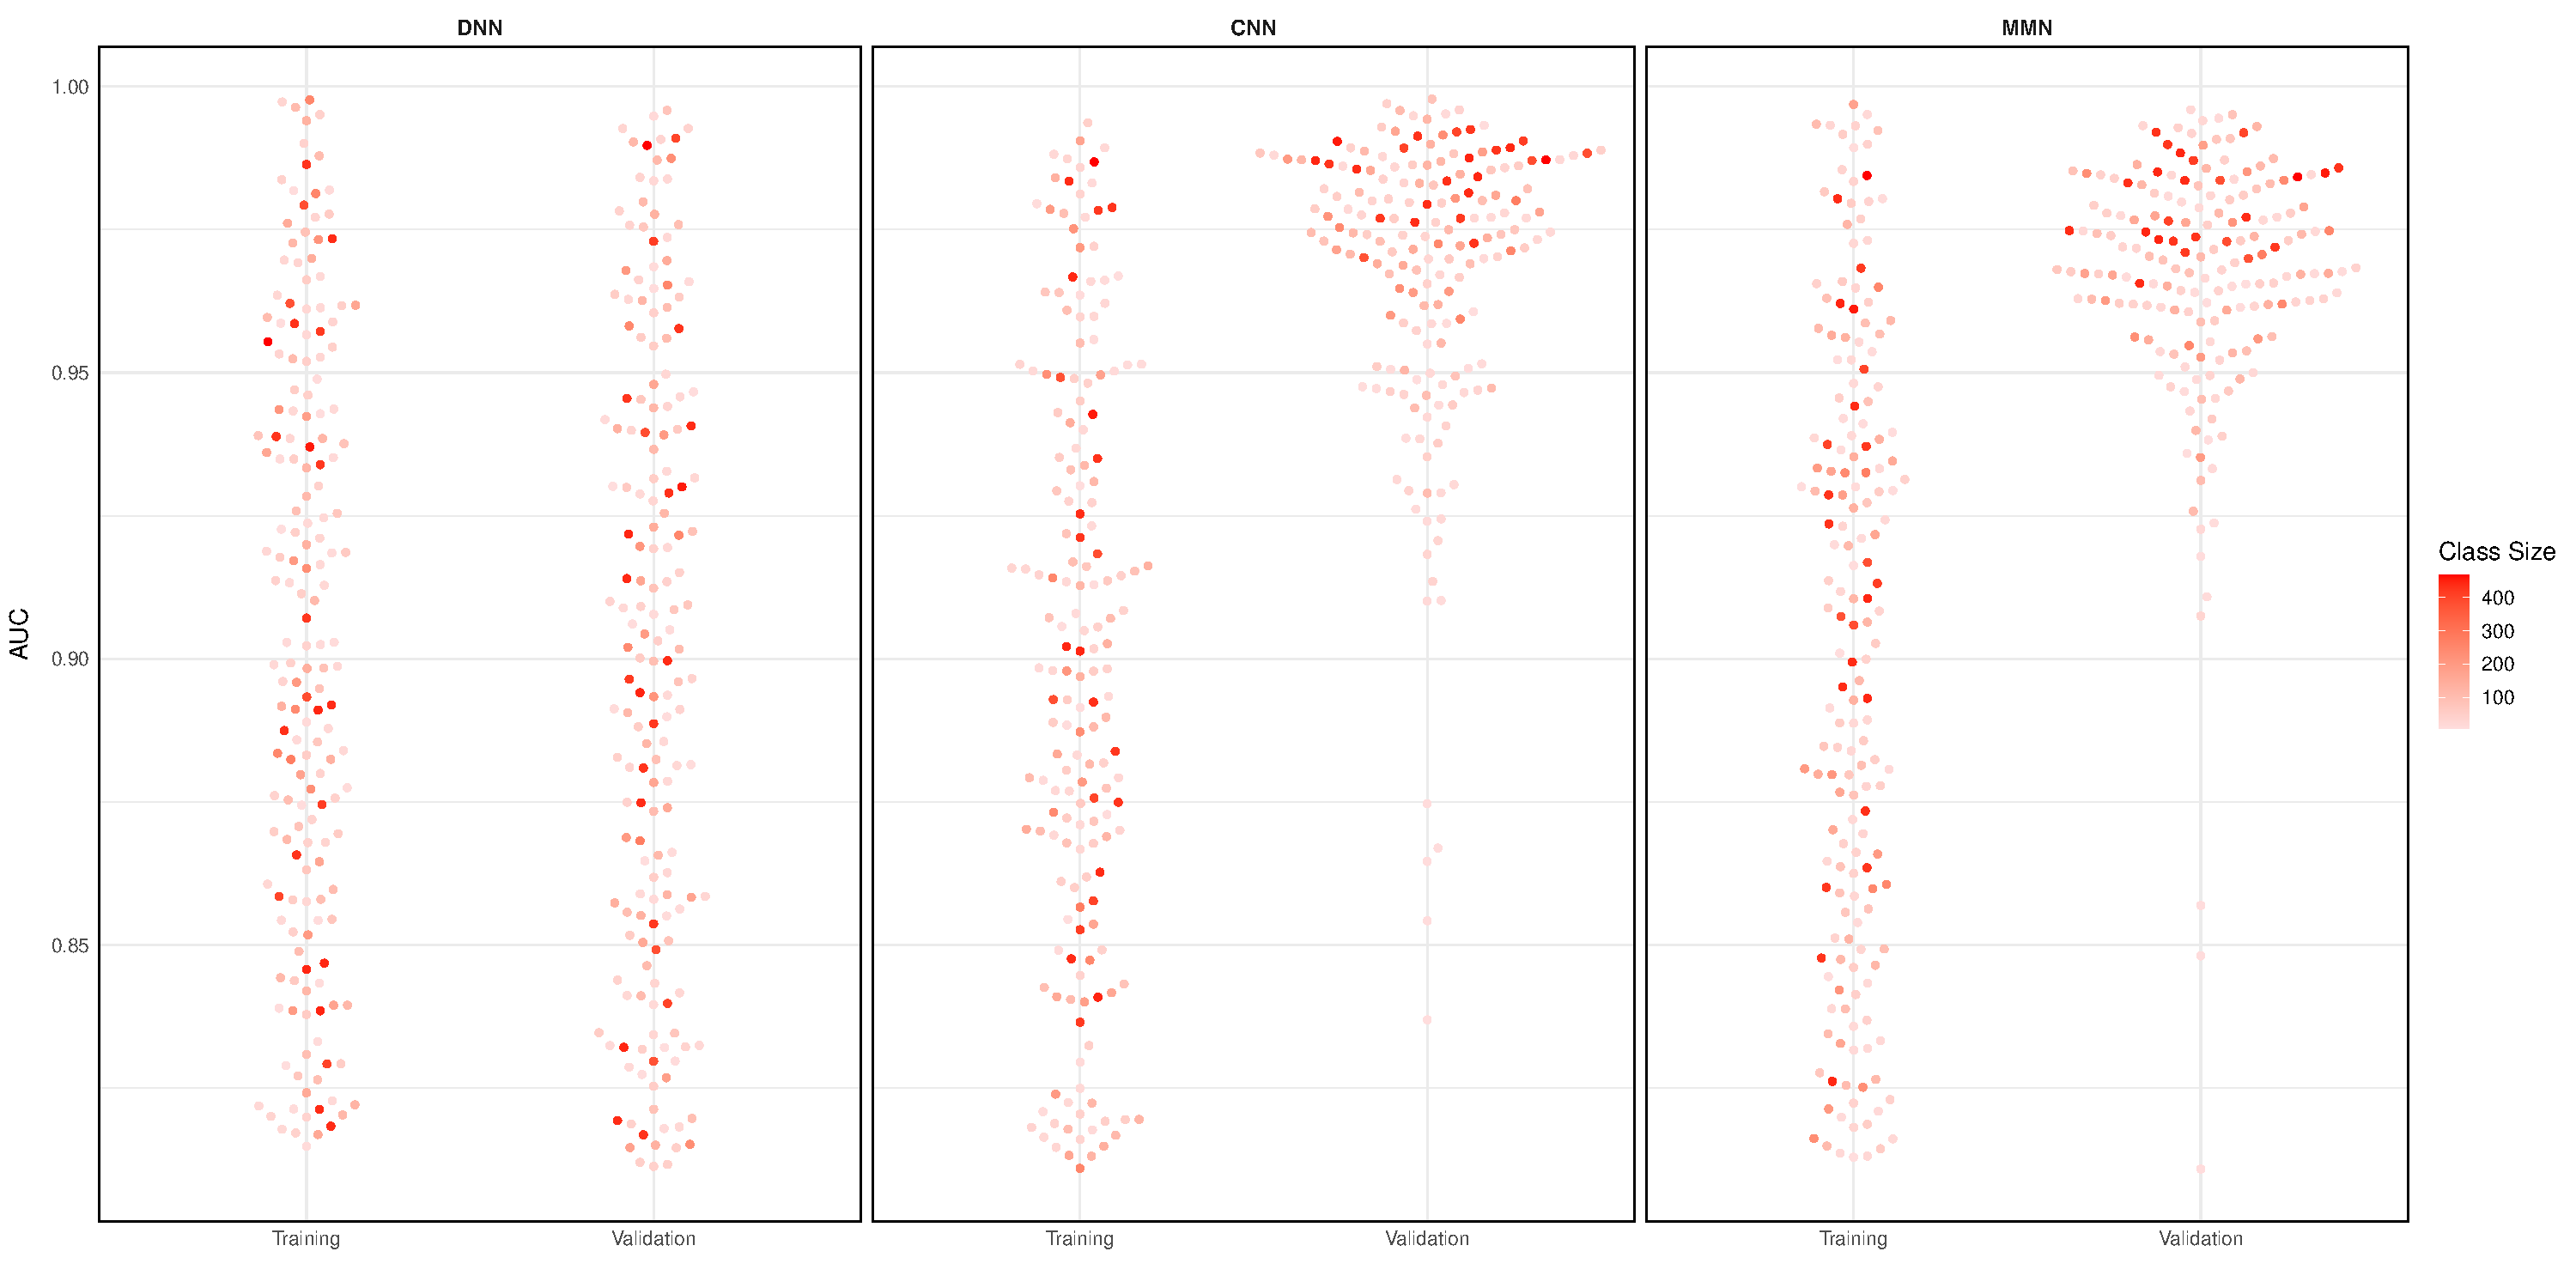
\includegraphics[width=\textwidth]{../analysis/results/figures/auc_beehive.pdf}
	\caption{Performance comparison of the three architectures implemented in \pkg{cito} (DNN, CNN, MMN) for bird species classification. DNNs were trained on the coordinates of the location of the audio recordings, CNNs were trained on the Mel spectrograms of the audio recordings, and MMNs were trained on both. Each architecture was trained 5 times in a 5-fold stratified cross-validation. For each of the 5 trained models, predictions were made for the 4 training folds, and the omitted validation fold. The predictions of the 5 models were combined to calculate two one-vs-all AUC values for each of the 177 bird species; one for the training and one for the validation predictions. These AUC values are shown, color coded according to the number of samples in the dataset belonging to the species.}
	\label{beehive}
	\vspace{1cm}
	\resizebox{\textwidth}{!}{\usebox{\cnn}}
	\newpage
\end{figure}

%\begin{figure}[h]
%	\centering
%	\resizebox{\textwidth}{!}{\usebox{\cnn}}
%\end{figure}


To demonstrate the transfer learning option, I used the MobileNet V2 \citep{sandlerMobileNetV2InvertedResiduals2019} architecture with pre-trained weights for the CNNs (and the CNN part of the MMNs). I set device = "cuda" to enable training on GPUs and changed the batchsize to 16, as the GPUs I used did not have enough memory to support the default batchsize of 32. I also set validation=0.1 and early\_stopping=3. This causes the models to use 10\% of the provided training data as a validation set and to stop training early if the loss on that validation set has not improved over the last 3 epochs, which not only reduces the training time of these models but also helps to reduce overfitting.

When comparing the performance of the architectures (Figure \ref{beehive}), I found that the CNN architecture performed better than the DNN and MMN.


\chapter*{Discussion and conclusion}
\addcontentsline{toc}{chapter}{Discussion and conclusion}
In this work, I presented the implementation of CNN and MMN architectures in the R package \pkg{cito}. Building and training CNNs previously required users to have extensive knowledge of complex deep learning frameworks such as PyTorch or TensorFlow. With the simple interface I provide, this is no longer necessary. Because of the \pkg{torch} backend and the GPU support it provides, \pkg{cito} can train these large networks as efficiently as the complex frameworks. I also provide the ability to use transfer learning by integrating several pre-trained models. To address the current trend towards multimodal models, I have implemented an MMN architecture that can combine the two neural network architectures currently available in \pkg{cito} (DNN and CNN). Using bird species classification as an example, I demonstrated how little code is required when using \pkg{cito} to train good performing CNN-based classifiers.

In my case study, the CNN achieved a high macro-average AUC of 0.967 on the validation sets of the 5-fold cross-validation. However, these results cannot be compared to the results of the Kaggle competition, as the models of the were evaluated on a separate test set, which has significant differences from the training set I performed my cross-validation on: 1) The test set contains only the audio files, not the coordinates. This makes it impossible to evaluate the DNNs and MMNs I trained on the test set, as they need these to make predictions. 2) Unlike the training set, which contains sound recordings from all over the world, the test set only contains sound recordings from the Western Ghats of India. This local blocking of the test set could reduce model performance, as a model trained on the global data could overfit to global patterns, such as background noise or local dialects of bird calls, that are not present in the local region of the test set. 3) The sound recordings in the test set have a fixed length of 4 minutes, whereas the median length of the sound recordings in the training set is only 22.7 seconds. A large proportion of the training recordings are shorter or only slightly longer than 10 seconds, so it can be expected that the randomly sampled 10-second chunk will contain at least parts of the bird call that can be used for prediction. The probability that a random 10-second chunk of the 4-minute audio recordings in the test set will contain parts of the bird call, rather than just noise, is lower. The winning team in the Kaggle competition dealt with this problem by dividing the audio recordings into 10-second chunks and then averaging the predictions of these chunks. As there may be chunks with little or no parts of the bird call and mostly background noise, this can increase the uncertainty of the final predictions and reduce the overall performance measured by AUC. 

The DNN and MMN architectures (Macro-averaged AUC: , respectively) performed worse than the CNN. For the DNN this was expected, since it only predicts on longitude and latitude values, which obviously aren't enough for a complex task such as species classification, because several different bird species can occur at the same location. However, I expected that the MMN which uses both the audio recordings and the coordinates might be better in detecting local dialects of the bird calls and, thus, achieve better results than the CNN. 

% Case study results:
%	- DNN und MMN vielleicht schlechter weil keine vortrainierten gewichte
%	- insbesondere da kein tuning (hyperparameter, architecture)

% mlr3torch
% - fuer machine learner, meins fuer oekologen
% - trochvision pretrained models verfuegbar
% - kein einfaches interface fuer custom CNNs

% Limitations of 'cito' and future work
%	- Transfer learning for 1D and 3D convolutions
% 	- XAI
% 	- Transposed convolutional layer ?
%	- other architectures: RNNs

% Conclusion:
%	- CNNs more accessible to researchers/ecologists



\newpage
\renewcommand{\bibname}{References}
\addcontentsline{toc}{chapter}{References} % Add Bibliography to the table of contents
% this is the style file. If you need to change something, google if the file you need is already there. If not (very uncommon) google makebst.
\bibliographystyle{chicago} 
\bibliography{../literature/literature} % Reference the BibTeX library file

\chapter*{Appendix}
\addcontentsline{toc}{chapter}{Appendix}
\lstdefinestyle{Rstyle}{
	language=R,
	basicstyle=\ttfamily\small,
	commentstyle=\color{green!60!black},
	stringstyle=\color{orange},
	showstringspaces=false,
	breaklines=true,
	frame=single,
	numbers=left,
	numberstyle=\tiny\color{gray},
	literate={/}{/}{1}  % Make "/" regular
			 {_}{\_}{1} % Make "_" regular
}
\lstset{style=Rstyle}
\section*{1-dataPreparation.R}
\lstinputlisting{../analysis/1-dataPreparation.R}
\newpage
\section*{2-buildingDNNs.R}
\lstinputlisting{../analysis/2-buildingDNNs.R}
\newpage
\section*{2-buildingCNNs.R}
\lstinputlisting{../analysis/2-buildingCNNs.R}
\newpage
\section*{2-buildingMMNs.R}
\lstinputlisting{../analysis/2-buildingMMNs.R}
\newpage
\section*{3-visualisation.R}
\lstinputlisting{../analysis/3-visualisation.R}
\newpage
\section*{utils.R}
\lstinputlisting{../analysis/utils.R}
\newpage

\chapter*{Declaration of independence}
\addcontentsline{toc}{chapter}{Declaration of independence}
Ich habe die Arbeit selbstständig verfasst, keine anderen als die angegebenen Quellen und Hilfsmittel benutzt und bisher keiner anderen Prüfungsbehörde vorgelegt. Außerdem bestätige ich hiermit, dass die vorgelegten Druckexemplare und die vorgelegte elektronische Version der Arbeit identisch sind, dass ich über wissenschaftlich korrektes Arbeiten und Zitieren aufgeklärt wurde und dass ich von den in §26 Abs. 5 vorgesehenen Rechtsfolgen Kenntnis habe.

\vspace{2cm}
\begin{flushright}
	\renewcommand{\arraystretch}{1.3}
	\begin{tabular}{ccc}
		\hline
		\hspace*{2cm}&Unterschrift&\hspace*{2cm}\\
	\end{tabular}
\end{flushright}


% Note: all files can be anywhere, just give the full path.


\end{document}
